%% ------------------------------------------------------------------------- %%
\chapter{Desenvolvimento Experimental}
\label{cap:desenvolvimentos}

Este trabalho tem o objetivo de desenvolver uma solução que seja capaz de remover a contaminação telúrica de espectros astronômicos capturados a partir do solo. Para fazer isso é necessário um conhecimento extenso sobre os dados coletados, desde como foram criados e compostos até sua semântica e nuances astronômicas.  

Neste capítulo são descritos os dados utilizados e os experimentos realizados durante o desenvolvimento do trabalho. Os experimentos foram úteis para compreender e visualizar os espectros de ciência e telúrico, testar o realinhamento de sinais e aprender características fundamentais dos espectros na solução do problema da contaminação telúrica.  

\section{Formato de dados}

% o que é o formato fits
O formato de dados utilizado nos experimentos é o FITS ou \textit{Flexible Image Transfer System}. Este formato de arquivo digital facilita o armazenamento, processamento e transmissão de dados científicos e foi projetado para armazenar conjuntos de dados $n$-dimensionais que consistem em matrizes e tabelas. Este é o formato de dados mais utilizado na astronomia, e inclusive possui recursos adicionais para incluir informações de calibração fotométrica e espacial e metadados de origem do arquivo \citep{pence2010definition}.

% composição do arquivo fits
Um arquivo FITS é composto por segmentos chamados de HDU (\textit{Header-Data Units}) e ele deve necessariamente ter um \textit{Primary HDU}, que armazena os dados científicos principais. O \textit{PrimaryHDU} pode ser acompanhado de HDUs adicionais, categorizados entre extensões de imagens, extensões de tabelas ASCII e extensões de tabelas binárias \citep{nasa-fits}.

% header
O \textit{header} de um arquivo FITS contém uma lista de palavras-chave em letra maiúscula, associadas a um valor e possivelmente seguidas de um comentário. Estas palavras-chave representam elementos dos dados que são importantes, como a data de observação do arquivo, seu autor, seu histórico de processamento, seu telescópio de origem e também podem representar elementos relacionados à física da observação, como a massa de ar no momento e local de observação, temperatura ambiente, umidade e etc.

\begin{figure}[htb]
\centering
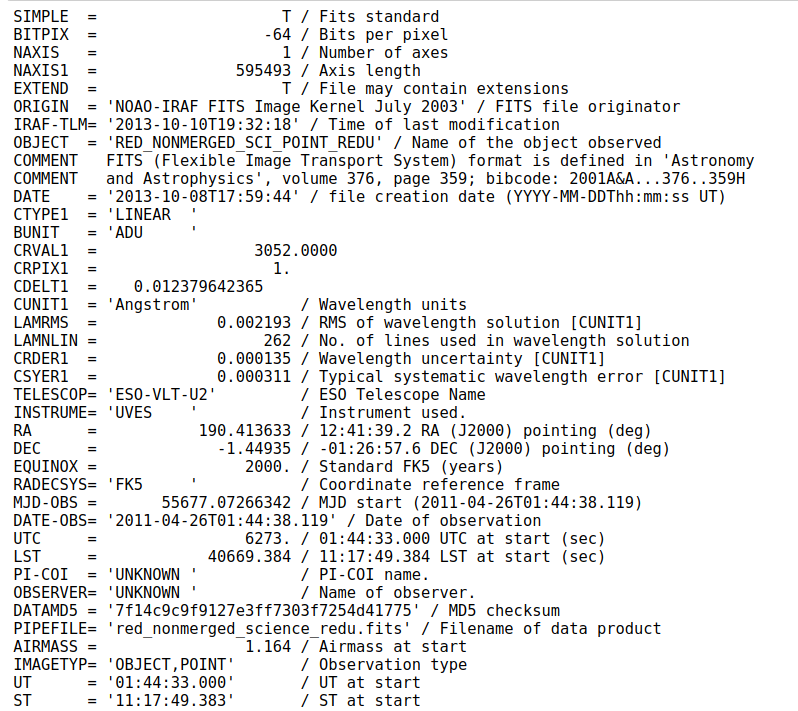
\includegraphics[width=10cm]{figuras/fits_header.png}
\caption{Trecho do cabeçalho do arquivo FITS da estrela HD110379}
\label{fig:fits-header}
\end{figure}

% data e tipos de dados
O componente em sequência do cabeçalho, quando presente, possui um vetor que pode ter desde 1 a 999 dimensões. Esta seção representa o dado astronômico capturado, como os valores do fluxo de um espectro estelar ou uma imagem de um objeto celeste. Os dados podem ter um de 5 possíveis tipos de dados \citep{pence2010definition}:

\begin{enumerate}
    \item Inteiros de 8 bits
    \item Inteiros de 16 bits
    \item Inteiros de 32 bits
    \item Números reais de ponto flutuante de 32 bits
    \item Números reais de ponto flutuante de 64 bits
\end{enumerate}

\section{Conjuntos de dados}

Para o desenvolvimento dos experimentos destre trabalho, foram fornecidos alguns conjuntos de dados estelares. Todos os arquivos destes conjuntos estão no formato FITS.

% datasets fornecidos: ardata, uves, molecfit e xsl (principal conjunto de dados)
Os conjuntos de dados estelares fornecidos englobam tanto observações reais de estrelas quando espectros telúricos sintéticos. Algumas das observações reais são: uma tabela FITS com observações reais do Sol, de Arcturus e de um referencial telúrico para ambos; dois pares de arquivos FITS contendo as estrelas de ciência HD110379 e HD110379 e seus respectivos referenciais telúricos, que foram capturadas pelo espectrógrafo UVES \footnote{\url{https://www.eso.org/sci/facilities/paranal/instruments/uves.html}} \citep{2000SPIE.4008..534D}, parte do \textit{Very Large Telescope Array} \footnote{\url{https://www.eso.org/public/brazil/teles-instr/paranal-observatory/vlt/?lang}}, no Cerro Paranal, Chile.  

% seleção do xsl como dataset principal
Porém, como foi mencionado na seção ~\ref{similarity-and-signal-alignment}, o principal conjunto de dados utilizado nos experimentos deste trabalho são estrelas do \textit{X-Shooter Spectral Library} \citep{Chen2014TheXS}, outro espectrógrafo que compõe o \textit{Very Large Telescope Array}. O diferencial deste conjunto de dados é que além das observações estelares e referenciais telúricos, foram fornecidos os espectros resultantes da correção telúrica. Desta maneira, foi possível estabelecer um \textit{ground truth} como base de comparação para os resultados dos experimentos.

% leitura dos dados
Mas antes de qualquer teste foi necessário um processo de conhecimento e ambientação com os dados astronômicos. Para leitura e manipulação de dados no formato FITS foi usada a biblioteca \textit{Astropy}\footnote{\url{http://www.astropy.org}}, que é amplamente usado para processar computacionalmente diversos dados astronômicos \citep{astropy:2018}. 

% exemplos de estrelas mencionadas acima
Com a combinação dos dados fornecidos e o ferramental correto, foi possível abrir, analisar e visualizar o espectro de diversas estrelas. Dois exemplos de estrelas de ciência e seus referenciais telúricos estão nas figuras ~\ref{fig:two-stars-hd110379} e ~\ref{fig:two-stars-sun}, e representam, respectivamente, a estrela HD110379 e o Sol.

% observado e o telurico de cada um (ardata e uves)
\begin{figure}[htb]
  \centering
  \subfloat[Sol]{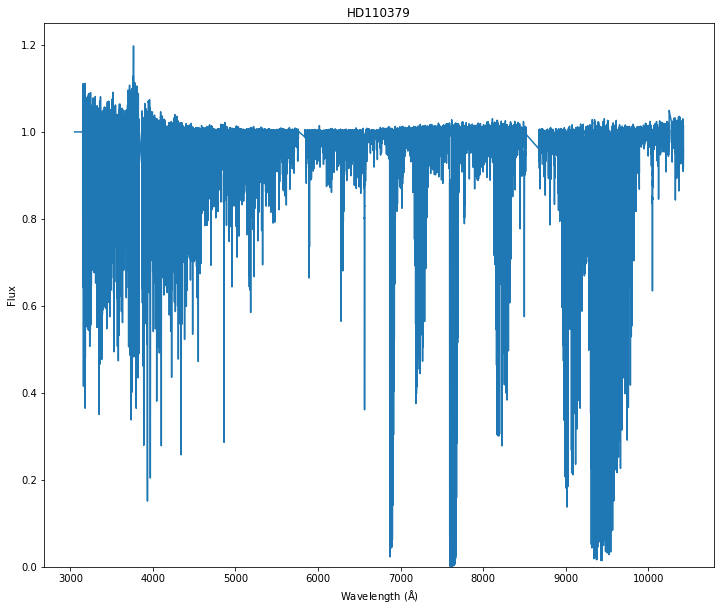
\includegraphics[width=0.5\textwidth]{figuras/hd110379_spectrum.png}\label{fig:hd110379}}
  \hfill
  \subfloat[Referência telúrica para HD110379]{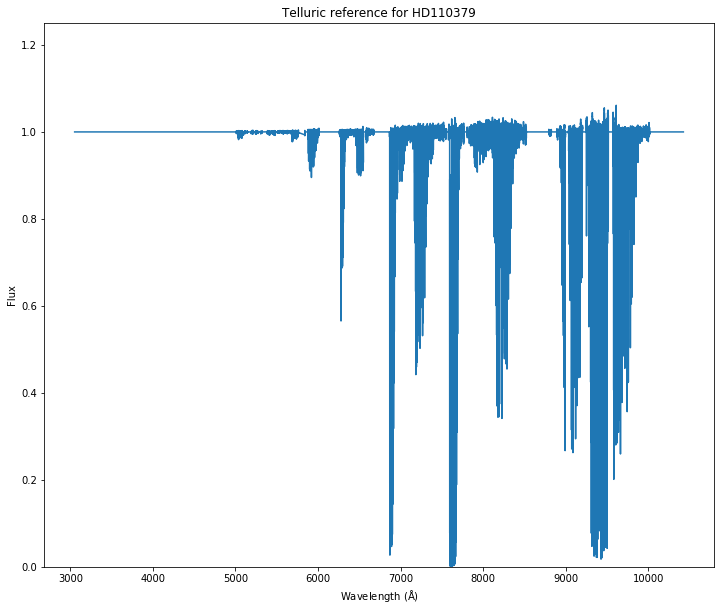
\includegraphics[width=0.5\textwidth]{figuras/hd110379_telluric.png}\label{fig:hd110379-tel}}
  \caption{Estrela de ciência e telúrica HD110379}
  \label{fig:two-stars-hd110379}
\end{figure}

\begin{figure}[htb]
  \centering
  \subfloat[Sol]{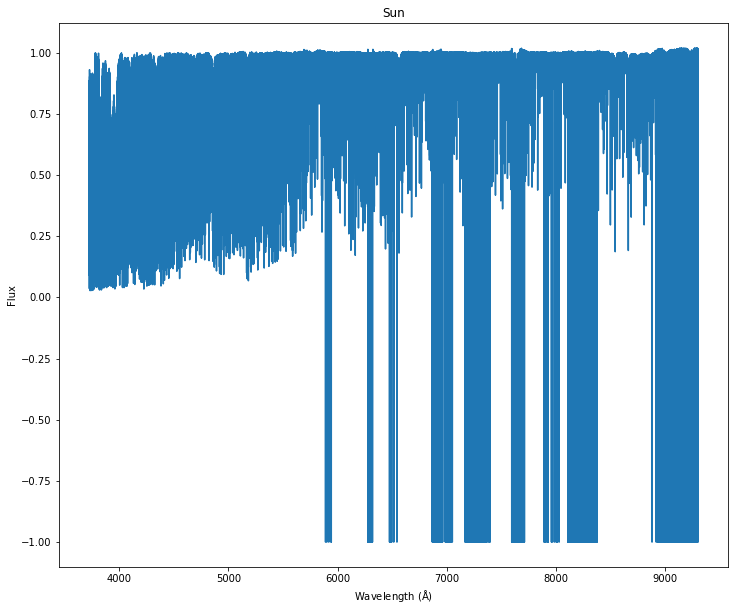
\includegraphics[width=0.5\textwidth]{figuras/sun_spectrum.png}\label{fig:sun}}
  \hfill
  \subfloat[Referência telúrica para o Sol]{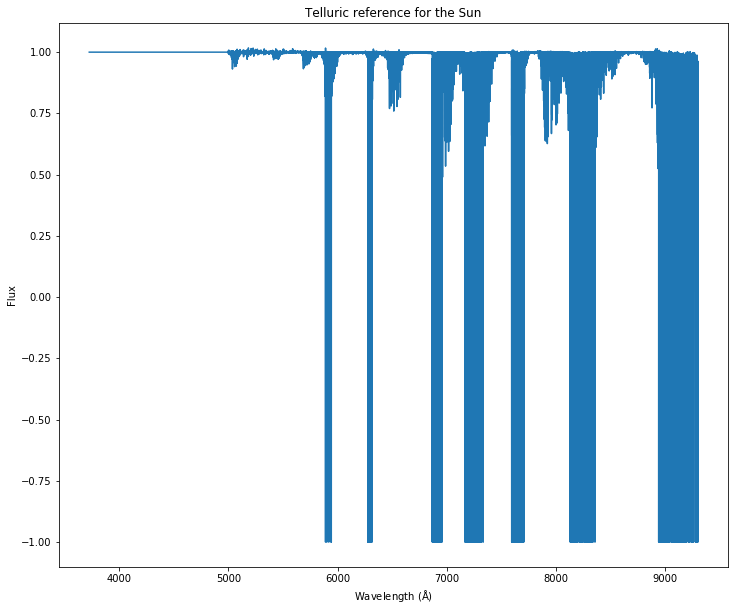
\includegraphics[width=0.5\textwidth]{figuras/sun_telluric.png}\label{fig:sun-tel}}
  \caption{Estrela de ciência e telúrica do Sol}
  \label{fig:two-stars-sun}
\end{figure}

% espectros e suas diferenças (formato do espectro, fonte, normalização, etc)
É possível observar nestas figuras que características dos espectros são alteradas devido à diferença de suas fontes e processo de redução de dados, ou seja, o dado espectral é relativo ao seu instrumento de observação e processamento consequente. Analogamente, é possível ver que conjuntos de dados da mesma fonte (par estrela de ciência e telúrica) possuem formatos similares.

% talvez seria mais interessante plotar os espectros nas unidades que vieram e depois mostrar que é possível interpolar os sinais para o intervalo de comprimento de onda correto usando dados do cabeçalho (fazer amanhã)

\section{Divisão do sinal estelar pelo telúrico}



\section{DTW no sinal estelar}

\section{DTW no sinal atmosférico}